%%%%%%%%%%%%%%%%%%%%%%%%%%%%%%%%%%%%%%%%%
% Beamer Presentation
% LaTeX Template
% Version 1.0 (10/11/12)
%
% This template has been downloaded from:
% http://www.LaTeXTemplates.com
%
% License:
% CC BY-NC-SA 3.0 (http://creativecommons.org/licenses/by-nc-sa/3.0/)
%
%%%%%%%%%%%%%%%%%%%%%%%%%%%%%%%%%%%%%%%%%

%----------------------------------------------------------------------------------------
%	PACKAGES AND THEMES
%----------------------------------------------------------------------------------------

\documentclass[aspectratio=169, xcolor=table]{beamer}

\mode<presentation> {

% The Beamer class comes with a number of default slide themes
% which change the colors and layouts of slides. Below this is a list
% of all the themes, uncomment each in turn to see what they look like.

%\usetheme{default}
%\usetheme{AnnArbor}
%\usetheme{Antibes}
%\usetheme{Bergen}
%\usetheme{Berkeley}
%\usetheme{Berlin}
%\usetheme{Boadilla}
%\usetheme{CambridgeUS} % XXX
%\usetheme{Copenhagen}
%\usetheme{Darmstadt}
%\usetheme{Dresden}
\usetheme{Frankfurt} % XXX
%\usetheme{Goettingen}
%\usetheme{Hannover}
%\usetheme{Ilmenau}
%\usetheme{JuanLesPins}
%\usetheme{Luebeck}
%\usetheme{Madrid}
%\usetheme{Malmoe}
%\usetheme{Marburg}
%\usetheme{Montpellier}
%\usetheme{PaloAlto}
%\usetheme{Pittsburgh}
%\usetheme{Rochester}
%\usetheme{Singapore} % XXX
%\usetheme{Szeged}
%\usetheme{Warsaw}

% As well as themes, the Beamer class has a number of color themes
% for any slide theme. Uncomment each of these in turn to see how it
% changes the colors of your current slide theme.

%\usecolortheme{albatross}
%\usecolortheme{beaver} % XXX
\usecolortheme{beetle} % XXX
%\usecolortheme{crane}
%\usecolortheme{dolphin}
%\usecolortheme{dove}
%\usecolortheme{fly} % XXX
%\usecolortheme{lily}
%\usecolortheme{orchid}
%\usecolortheme{rose}
%\usecolortheme{seagull}
%\usecolortheme{seahorse}
%\usecolortheme{whale}
%\usecolortheme{wolverine}

%\setbeamertemplate{footline} % To remove the footer line in all slides uncomment this line
\setbeamertemplate{footline}[page number] % To replace the footer line in all slides with a simple slide count uncomment this line

\setbeamertemplate{navigation symbols}{} % To remove the navigation symbols from the bottom of all slides uncomment this line
}

\usepackage{graphicx} % Allows including images
\usepackage{booktabs} % Allows the use of \toprule, \midrule and \bottomrule in tables
\usepackage[utf8]{inputenc}
\usepackage{hyperref}
\usepackage{wasysym}
\usepackage{tikz}
\usepackage[table]{xcolor}
\usepackage{lipsum}
%\usepackage[table,xcdraw]{xcolor}

% \setlength{\arrayrulewidth}{1mm}
% \setlength{\tabcolsep}{18pt}
% \renewcommand{\arraystretch}{2.5}

\makeatletter
\pgfkeys{/pgf/.cd,
  parallelepiped offset x/.initial=2mm,
  parallelepiped offset y/.initial=2mm
}
\pgfdeclareshape{parallelepiped}
{
  \inheritsavedanchors[from=rectangle] % this is nearly a rectangle
  \inheritanchorborder[from=rectangle]
  \inheritanchor[from=rectangle]{north}
  \inheritanchor[from=rectangle]{north west}
  \inheritanchor[from=rectangle]{north east}
  \inheritanchor[from=rectangle]{center}
  \inheritanchor[from=rectangle]{west}
  \inheritanchor[from=rectangle]{east}
  \inheritanchor[from=rectangle]{mid}
  \inheritanchor[from=rectangle]{mid west}
  \inheritanchor[from=rectangle]{mid east}
  \inheritanchor[from=rectangle]{base}
  \inheritanchor[from=rectangle]{base west}
  \inheritanchor[from=rectangle]{base east}
  \inheritanchor[from=rectangle]{south}
  \inheritanchor[from=rectangle]{south west}
  \inheritanchor[from=rectangle]{south east}
  \backgroundpath{
    % store lower right in xa/ya and upper right in xb/yb
    \southwest \pgf@xa=\pgf@x \pgf@ya=\pgf@y
    \northeast \pgf@xb=\pgf@x \pgf@yb=\pgf@y
    \pgfmathsetlength\pgfutil@tempdima{\pgfkeysvalueof{/pgf/parallelepiped offset x}}
    \pgfmathsetlength\pgfutil@tempdimb{\pgfkeysvalueof{/pgf/parallelepiped offset y}}
    \def\ppd@offset{\pgfpoint{\pgfutil@tempdima}{\pgfutil@tempdimb}}
    \pgfpathmoveto{\pgfqpoint{\pgf@xa}{\pgf@ya}}
    \pgfpathlineto{\pgfqpoint{\pgf@xb}{\pgf@ya}}
    \pgfpathlineto{\pgfqpoint{\pgf@xb}{\pgf@yb}}
    \pgfpathlineto{\pgfqpoint{\pgf@xa}{\pgf@yb}}
    \pgfpathclose
    \pgfpathmoveto{\pgfqpoint{\pgf@xb}{\pgf@ya}}
    \pgfpathlineto{\pgfpointadd{\pgfpoint{\pgf@xb}{\pgf@ya}}{\ppd@offset}}
    \pgfpathlineto{\pgfpointadd{\pgfpoint{\pgf@xb}{\pgf@yb}}{\ppd@offset}}
    \pgfpathlineto{\pgfpointadd{\pgfpoint{\pgf@xa}{\pgf@yb}}{\ppd@offset}}
    \pgfpathlineto{\pgfqpoint{\pgf@xa}{\pgf@yb}}
    \pgfpathmoveto{\pgfqpoint{\pgf@xb}{\pgf@yb}}
    \pgfpathlineto{\pgfpointadd{\pgfpoint{\pgf@xb}{\pgf@yb}}{\ppd@offset}}
  }
}
\makeatother
\renewcommand{\thefootnote}{\fnsymbol{footnote}} % numeración por símbolos
%----------------------------------------------------------------------------------------
%	TITLE PAGE
%----------------------------------------------------------------------------------------

\title[Tíulo corto]{Título de la presentación\\ \underline{ \textit{Evento muy importante}} } % The short title appears at the bottom of every slide, the full title is only on the title page

\author{Pepe Pecas} % Your name
\institute[Universidad] % Your institution as it will appear on the bottom of every slide, may be shorthand to save space
{
Universidad muy importante\\
Institución muy importante\\ % Your institution for the title page
%\medskip
\textit{john@smith.com} % Your email address
}
\date{ 21 / Julio / 2023} % Date, can be changed to a custom date

\begin{document}

\begin{frame}

 \begin{center}
 \includegraphics[width=0.13\textwidth]{./img/logo1.png}\hspace{10cm}%\hspace{3.8cm}
 \includegraphics[width=0.13\textwidth]{./img/logo2.png}
 \end{center}

\titlepage % Print the title page as the first slide
\end{frame}

%----------------------------------------------------------------------------------------
%	PRESENTATION SLIDES
%----------------------------------------------------------------------------------------

%------------------------------------------------
\section{Introducción}

\begin{frame}\frametitle{Lorem ipsum in dolo }

  \lipsum[1][1]
  
  \begin{itemize}
   \item item1.
   \item item2.
   \item item3 con valor US\$ $24, 769, 420$.
  \end{itemize}

\end{frame}

\begin{frame}\frametitle{Lorem ipsum in dolo}
  
  \lipsum[1][2]
  
  \begin{center}
    \includegraphics[width=0.45\textwidth]{./img/a1.png}\
    \includegraphics[width=0.45\textwidth]{./img/b2.png}
  \end{center}
\end{frame}

\section{Objetivo}
\begin{frame}\frametitle{Lorem ipsum in dolo}
  \lipsum[1][1-3]
\end{frame}

\section{Marco teórico}
\begin{frame}\frametitle{Lorem ipsum in dolo}
  \lipsum[1][1-3]
\end{frame}

\begin{frame}\frametitle{Esto se hizo con TikZ}
    \begin{center}
    \centering \includegraphics[width=0.15\textwidth]{./img/a1.png}\
    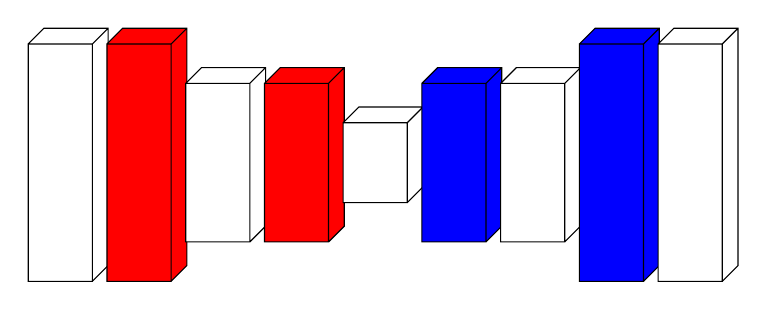
\begin{tikzpicture}
    
%     \node[parallelepiped,draw=black,fill=white,
%       minimum width=.4cm,minimum height=2cm] (1) {};
%       
%     \node[parallelepiped,draw=black,fill=red,
%     minimum width=.4cm,minimum height=2cm] (2)
%     at (.5,0) {};
    
    \node[parallelepiped,draw=black,fill=white,
      minimum width=.8cm,minimum height=3cm] (3)
      at (1,0) {};
      
    \node[parallelepiped,draw=black,fill=red,
    minimum width=.8cm,minimum height=3cm] (4)
    at (2,0) {};
    
    \node[parallelepiped,draw=black,fill=white,
      minimum width=.8cm,minimum height=2cm] (5) 
      at (3,0) {};
      
    \node[parallelepiped,draw=black,fill=red,
    minimum width=.8cm,minimum height=2cm] (6)
    at (4,0) {};
    
    \node[parallelepiped,draw=black,fill=white,
      minimum width=.8cm,minimum height=1cm] (7) 
      at (5,0) {};
    
    \node[parallelepiped,draw=black,fill=blue,
      minimum width=.8cm,minimum height=2cm] (8) 
      at (6,0) {};
      
    \node[parallelepiped,draw=black,fill=white,
    minimum width=.8cm,minimum height=2cm] (9)
    at (7,0) {};
    
    \node[parallelepiped,draw=black,fill=blue,
      minimum width=.8cm,minimum height=3cm] (10) 
      at (8,0) {};
      
    \node[parallelepiped,draw=black,fill=white,
    minimum width=.8cm,minimum height=3cm] (11)
    at (9,0) {};
    
%     \node[parallelepiped,draw=black,fill=blue,
%     minimum width=.4cm,minimum height=2cm] (12) 
%     at(5.5,0){};
%       
%     \node[parallelepiped,draw=black,fill=white,
%     minimum width=.4cm,minimum height=2cm] (13)
%     at (6,0) {};
    
    \end{tikzpicture}
    \centering \includegraphics[width=0.15\textwidth]{./img/a1-r.png}
    
  \end{center}
\end{frame}

\section{Metodología}

\begin{frame}\frametitle{Lorem ipsum in dolo}
  \lipsum[1]
\end{frame}

\section{Resultados}

\begin{frame}\frametitle{\textbf{Lorem ipsum} in dolo }
  
  \begin{center}
  
    \rotatebox{90}{Uno} \
    \includegraphics[width=0.145\textwidth]{./img/a1.png}\
    \includegraphics[width=0.145\textwidth]{./img/b2.png}\
    \includegraphics[width=0.145\textwidth]{./img/logo2.png}\\
    
    \rotatebox{90} {\footnotesize Dos} \
    \includegraphics[width=0.145\textwidth]{./img/a1-r.png}\
    \includegraphics[width=0.145\textwidth]{./img/b2-r.png}\
    \includegraphics[width=0.145\textwidth]{./img/logo1.png}\\
    
  \end{center}

\end{frame}

\end{document}

